\chapter{A Multi-Domain SDN for Dynamic Layer-2 Path Service}
\label{sec:DYNES}

The term ``domain'' is used to represent a network that is owned and operated by
a single organization, e.g., University of Virginia's domain, AT\&T's domain.
To establish and release layer-2 VLANs that traverse multiple domains requires sophisticated
control-plane operations.

\section{Introduction}

Over the past decade, the high-performance research-and-education (R\&E) networking
community that supports scientific computing has invested in developing architectures,
protocols, and
software controllers to support rate-guaranteed
dynamic Layer-2 (L2) path services \cite{1541694,4444698,4374315,1497551,4146687,OSCARS,OESS,1742-6596-396-4-042065}.
Applications include
(i) large dataset transfers \cite{UVA-CTRQ2013},
(ii) reliable multicast of file stream \cite{ji2015file},
(iii) high-rate delay-sensitive interactive
applications such as remote visualization and remote
instrument control, and (iii) resource isolation in virtualized networks \cite{GENI}.

To support rate-guaranteed dynamic L2 path services,
two components are required. \emph{First},
switches/routers should have data-plane support for classifying packets into flows, policing flows on ingress ports to ensure that they do not exceed their rate allocations, and scheduling packets on egress ports according to their flow-rate allocations. \emph{Second}, control-plane support
is required for admission control to check whether sufficient bandwidth resources are available before accepting a path-setup request, provisioning the path prior to usage (which means setting label mappings in switches for data-plane packet forwarding), and releasing resources and label mappings upon completion of usage. The introduction of OpenFlow/SDN technologies reduces the barriers to deploying dynamic rate-guaranteed L2-path service since the required control-plane software can be implemented in an external SDN controller rather than in switches.

Considerable advances have been made in enabling dynamic L2-path service.
\emph{First}, control-plane protocols have been specified and are being standardized. These
include Inter-Domain Controller Protocol (IDCP) \cite{IDCP} and the
Open Grid Forum Network Service Interface Connection Services (NSI CS) version 2.0 \cite{NSI}. Both protocols support
inter-domain signaling for advance-reservation and provisioning of rate-guaranteed
dynamic L2 paths. \emph{Second}, Internet2 and ESnet, the two major US backbone Research-and-Education
Network (REN) providers, have
deployed SDN controllers and Layer-2 switches to
support dynamic L2 path service. These controllers
include Open Exchange Software Suite (OESS)\cite{OESS} and
On-Demand Secure Circuits and Advance Reservation System (OSCARS)\cite{OSCARS}. OESS is an intra-domain
SDN controller that controls switches via OpenFlow, while
OSCARS supports inter-domain service.

The \emph{contributions} of this work are that we leveraged an existing deployment
called Dynamic Network System (DYNES) \cite{1742-6596-396-4-042065}, in which small SDNs were deployed
in multiple university campuses and regional RENs, to test multi-domain dynamic L2 path service. This thesis
offers insights into the complex issues that we encountered in deploying OESS and OSCARS in multiple domains (organizations), and describes the problems we encountered while provisioning inter-domain dynamic L2 paths. These problems can be solved to continue growing this dynamic L2-path service. The work presented in this chapter was
published in ACM NDM 2015 \cite{tepsuporn2015multi}.

The \emph{novelty} of this work is that it reports on a multi-domain SDN service in
which an inter-SDN-controller protocol is used for cooperative dynamic L2-path reservation and provisioning. Prior papers on SDN, e.g., Google B4  \cite{Jain:2013:BEG:2486001.2486019} and Microsoft's SWAN \cite{Hong:2013:AHU:2486001.2486012} are single-domain deployments. The GENI stitching approach
\cite{GENI-stitching} uses a tree model
that is designed to support network researchers. Our objective is to create
a scalable solution for a broader range of use cases.
Previous work on DYNES \cite{1742-6596-396-4-042065} described the use of OSCARS, and data-plane experiments. Our work builds on this prior work and makes the new contributions listed above.

The \emph{impact} of this work can be far-reaching. Our dynamic L2 service deployment is comparable to the early ARPAnet deployment of IP-routed service in 1970, when there were fewer than 10 connected universities. Just as ARPAnet grew into today's Internet with its IP-routed (L3) service, our seed deployment of a multi-domain rate-guaranteed dynamic L2 path service reaching 8 campuses could grow into a global-scale service, offering an opportunity for new delay-sensitive applications that are not supported well on today's best-effort IP service.

Section~\ref{sec:control-plane} describes the control plane software OESS and OSCARS, the provisioning process of the integrated system.
Section~\ref{sec:mdsdn} describes our experience of equipment setup, OESS GUI for reserving an OpenFlow path, hosts configuration for path provisioning.
Section~\ref{sec:insights} describes the lessons we learned from the experiments, the scalability of the system, and the troubleshooting process.
Section~\ref{sec:mdvlan} describes my experiments from an inter-domain multi-point VLAN, basically the process of provisioning by AL2S OESS and data plane work. 



\section{Background}
\label{sec:control-plane}
This section describes the two control-plane software systems, OESS and OSCARS. OESS is an OpenFlow controller
that accepts user advance-reservation requests for L2 paths
(in which start time, rate, duration, and endpoints are specified), performs intra-domain path computation, and configures rules in the switches along the path for VLAN based
packet forwarding using OpenFlow. OSCARS performs similar functions, and additionally supports inter-domain path
reservations and provisioning. Also, it can communicate
with a variety of switches/routers including some that do not
implement OpenFlow. Both OSCARS and OESS offer users
a Web Browser User Interface (UI) and a programmatic Web Service Interface for applications. In this section, we briefly
review the functionality offered by these controllers.
OESS supports integration with OSCARS, specifically to support inter-domain circuits.

\subsection{On-Demand Secure Circuits and Advance Reservation System (OSCARS)}
We review the overall OSCARS architecture, describe how trust/peering relationships are established between neighbouring OSCARS, and how topology is discovered before presenting how OSCARS reserves resources and provisions and releases paths (which is its main role). We end with a short review of path computation, which is executed during resource reservation \cite{OSCARS}.

\paragraph{Software architecture}
The OSCARS software consists of 11 modules that have distinct functions such as authentication, authorization, path finding, messaging, hardware mediation, and process coordination. Today, OSCARS supports inter-domain L2 paths using both the Inter-Domain Controller Protocol (IDCP) \cite{IDCP} and Network Service Interface Connection Services (NSI CS) version 2.0 \cite{NSI} protocols. The authorization (i.e., policy enforcement) of guaranteed bandwidth reservation requests are domain specific and can be enforced using the policy path computation modules within the OSCARS v0.6 Path Computation Engine (PCE) framework.

\paragraph{Trust/peering relationships}
The current trust model for
inter-domain dynamic paths is based on transitive peer-to-peer authentication and authorization. This work-flow mimics the telecommunication industry model; neither require downstream providers to know anything about the originating caller.

\paragraph{Topology discovery}
Each domain is responsible for discovering and pushing its topology to the perfSONAR Topology Service (pS-TS). The distributed pS-TS maintains
global topology information, and OSCARS servers can pull
the latest information from pS-TS as needed in real-time.
Topology information must be formatted in either the Open
Grid Forum Network Markup Language (NML) \cite{van2013network} or the NM-Control Plane \cite{IDCP} schemas to support the NSI CS v2.0
and the IDCP protocols, respectively.

\paragraph{Inter-domain L2 path reservation, provisioning, and
release}
When the OSCARS server in a domain receives an inter-domain VC reservation request, it reserves resources within its
own domain and sends a \texttt{createReservation} message
with endpoints, rate, start time (advance-reservation support)
and duration, to the OSCARS in the next domain, which is
selected based on the computed path. The procedure is executed in a daisy-chain fashion, as shown in Fig.~\ref{fig:daisychain},
until the OSCARS of the last domain on
the end-to-end path is reached. If successful, \texttt{Confirmation}
events are sent from one domain’s OSCARS server to the next
in the reverse direction. Provisioning of the VC occurs either
automatically or upon receiving a \texttt{createPath} message
from the user just before the reservation start-time. This procedure also uses a daisy-chain of signaling messages between
OSCARS servers. Each OSCARS server communicates with
the switches in its domain to provision the VC across the
domain. Finally, when the reservation end-time is reached a
\texttt{teardownPath} message is sent in daisy-chained mode to
release the VC.

The current trust model for inter-domain dynamic paths is based on transitive peer-to-peer authentication and authorization. This work-flow mimics the telecommunication industry model; neither require downstream providers to know anything about the originating caller.
\begin{figure}
\centering
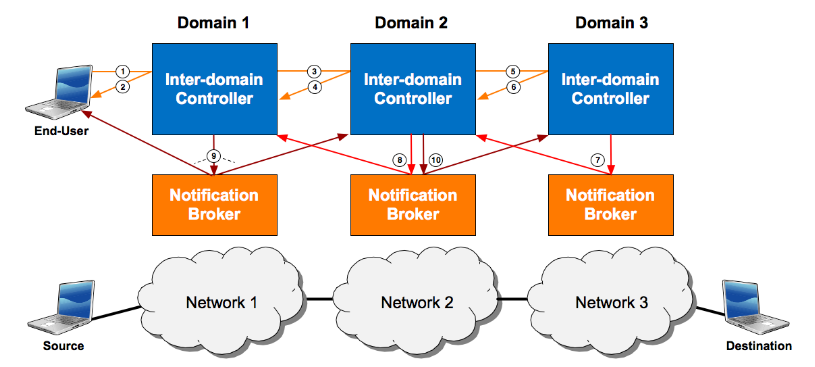
\includegraphics[width=0.6\textwidth]{figures/daisychain.png}
\caption{Daisy-chain model used by OSCARS for inter-domain circuit reservation, provisioning, and release}
\label{fig:daisychain}
\end{figure}

\paragraph{Path computation} In OSCARS v0.6, path computation
executed using ``atomic" Path Computation Engine (PCE) modules that can be
arbitrarily linked together. Each PCE module typically addresses a
specific constraint and prunes the graph accordingly. For example, a bandwidth PCE would discard all links that do not
have sufficient bandwidth, and a policy PCE would remove
all resources that the requester is not authorized to use.
While the PCE methods surveyed by Paolucci et al. \cite{6422287} are
for immediate-request paths, the OSCARS PCE supports
advance-reservation paths.


\subsection{Open Exchange Software Suite (OESS)}
\label{sec:OESS}

The Open Exchange Software Suite (OESS) is an OpenFlow
controller used to configure and control dynamic L2 paths
across a network of OpenFlow-enabled switches. OESS provides sub-second circuit provisioning, automatic circuit failover, per-interface permissions, and automatic per-VLAN
statistics.

\paragraph{OpenFlow path provisioning}
When a user wishes to provision an L2 path in OESS, the user must first select the endpoints (at least 2), rate, start time, duration, VLAN IDs, and optionally specify a path (with possibly a backup path) that connects all endpoints. In this context, endpoints are OpenFlow switch ports. For example, in Fig.~\ref{fig:oscarsoess}, consider the two numbered ports: port 19 of the DYNES switch in the University 1 network, and port 20 of the DYNES switch in the University 2 network. These two ports are the endpoints specified in a request for an end-to-end L2 path between the FDT hosts at University 1 and University 2.

Once the user has specified all the parameters in the request, the OESS UI sends the request to a Forwarding Controller. The Forwarding
Controller then calculates the \texttt{OFFlowMods}, which is a specification of the OpenFlow rules required to provision the path.
Each switch will receive at least 2 \texttt{OFFlowMods} (in cases of
multiPoint VLANs, there can be more than 2 \texttt{OFFlowMods}).
Each \texttt{OFFlowMod} is broken up into a \texttt{Match} and an \texttt{Action}.
The OpenFlow Match is applied to all packet headers, and
if a packet matches all of the fields in the OpenFlow \texttt{Match},
all of the OpenFlow \texttt{Actions} for the \texttt{OFFlowMod} are then
applied to the packet.

OESS has implemented a specific set
of OpenFlow \texttt{Matches} and \texttt{Actions}. All OESS \texttt{OFFlowMods}
for a VC consist of a \texttt{Match} that contains the input port
(\texttt{IN\_PORT}) and input VLAN ID (\texttt{DL\_VLAN}) fields. The
\texttt{Actions} consist of \texttt{SET\_VLAN\_ID} and OUTPUT (to a port)
actions. In some cases, the \texttt{STRIP\_VLAN} action is also used
(for untagged circuits). OESS uses NOX \cite{gude2008nox} to send \texttt{OFFlowMods} to the OpenFlow switches as shown in Fig.~\ref{fig:ControlPlane}.

In a network with QoS support, the controller would issue commands to configure filters, policing and scheduling in the OpenFlow switches so that flows do not violate the rates specified during path reservation. OpenFlow 1.3.0 supports QoS features, but the OESS implementation used in this study supported only OpenFlow 1.0 because Internet2 AL2S, for which OESS was initially designed, had only OpenFlow 1.0 switches when this study was carried out.

\paragraph{Topology discovery}
OESS learns the topology for its domain,
through a protocol similar to Link Layer Discovery Protocol (LLDP), called OpenFlow Discovery Protocol (OFDP) \cite{OFDP}.
OFDP functions by having the controller generate a packet
and send the packet out on every interface of an OpenFlow
switch using the \texttt{OFPacketOut} mechanism. The packet that
is sent out on each interface is tagged with the \texttt{DataPathID}
(a unique identifier for each OpenFlow Switch that is usually
based on a management MAC address) and number of the
interface on which the packet was sent. A rule is configured on
all switches to ``punt'' these topology-discovery packets to the
controller through an \texttt{OFPacketIn} event. The \texttt{OFPacketIn}
event sends the packet that arrived at the switch along with the
port and \texttt{DataPathID} of the switch that received the packet.
When this procedure occurs in both directions of an inter-switch link, an adjacency
is detected and OESS creates a link between the two devices on
the specified ports. OESS can also detects link failures and
node insertions, allowing for the OESS to automatically move
thousands of VLAN VCs with minimal human intervention.

% \paragraph{OESS software architecture}
% Fig.~\ref{fig:ControlPlane} shows the software architecture of OESS. OESS provisions an intra-domain circuit by using the NOX \cite{gude2008nox} API. NOX %is an OpenFlow controller that offers a programmatic interface to other controllers and applications. The module marked ``OSCARS''
% inside OESS is an interface to OSCARS. In addition to this interface, OESS has implemented
% a native module for NSI, the newer inter-domain control-plane protocol.

\begin{figure*}[htbp!]
\centering
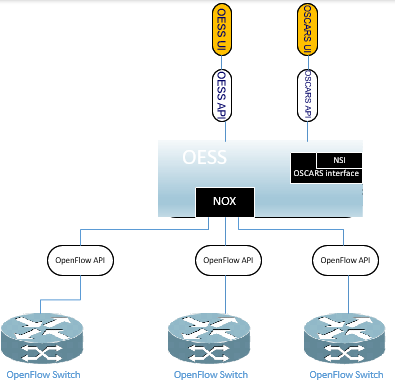
\includegraphics[width=0.6\textwidth]{figures/ControlPlane.PNG}
\caption{OESS software architecture}
\label{fig:ControlPlane}
\end{figure*}

\paragraph{OESS-OSCARS integration}
OESS includes an OSCARS interface module as shown in Fig.~\ref{fig:ControlPlane}. OESS automatically generates a
topology file for its domain and uploads it to the OSCARS
topology service as shown in Fig~\ref{fig:oscarsoess}. Only interfaces and VLAN IDs for which
users have granted OSCARS access appear in the OSCARS
topology file.

When a user requests an inter-domain circuit
via the OESS UI, the UI loads all topologies located in the
OSCARS topology service, and presents them to the user.
Once the endpoints have been selected and the user requests
that a VC be provisioned, the OESS UI submits a request to
OSCARS via the OSCARS SOAP API on behalf of the user.
At this point, the request has been turned over to OSCARS to
complete its path computation, and inform the other domains
of the request. When it is time for OSCARS to provision the
circuit in the local domain, it contacts the Path Setup Service
(PSS). When OESS is deployed in a domain, the OSCARS
PSS is replaced with the OESS PSS. The OESS PSS takes
the provisioning request from OSCARS, as shown in Fig~\ref{fig:oscarsoess}, and provisions an
OpenFlow path as described earlier. The OESS then reports the
success or failure of the provisioning procedure to OSCARS.
In cases where a user request for an inter-domain VC is sent
directly to OSCARS, the OESS PSS is nevertheless involved
to check the validity of the VC request and to carry out the
OpenFlow path provisioning.

\begin{figure}
\centering
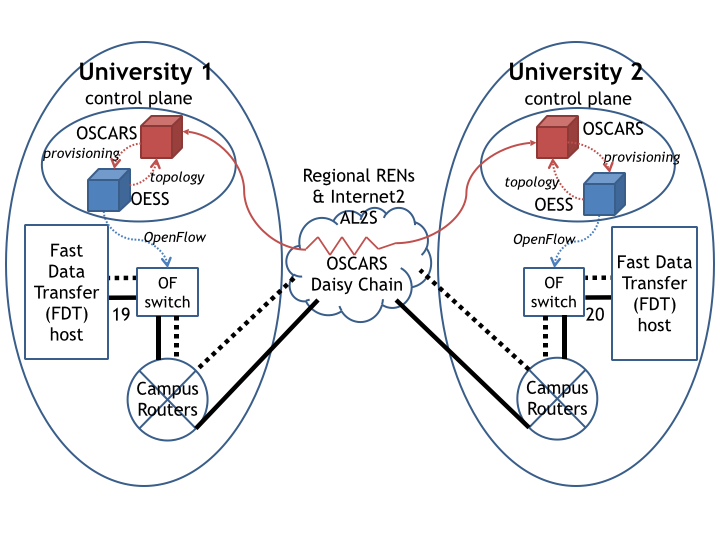
\includegraphics[width=0.6\textwidth]{figures/oscarsoess.png}
\caption{OSCARS and OESS integration}
\label{fig:oscarsoess}
\end{figure}


\section{Multi-domain SDN}
\label{sec:mdsdn}
Section~\ref{sec:multidomain-SDN-deploy-and-config} describes the equipment,
Section~\ref{sec:multidomain-SDN-path-provisioning} describes control-plane
operations for path provisioning, and Section~\ref{sec:multidomain-SDN-FDT-access} describes the actions required
in the hosts at the ends of an L2 path to support our use case (dataset transfers).
Section~\ref{sec:multidomain-SDN-data-plane-expts} describes a simple experiment
to test data-plane connectivity across the dynamically configured inter-domain L2 VLAN paths.

\subsection{Equipment}
\label{sec:multidomain-SDN-deploy-and-config}

In a project called Dynamic Network System (DYNES) \cite{1742-6596-396-4-042065}, distributed instruments were deployed in 40 universities and 11 regional RENs. Our work
used the DYNES instruments in the following universities:
(i) U. Virginia (UVA), (ii) MAX GigaPoP (MAX), (iii) U. Wisconsin, Madison (UWisc), (iv) University of New Hampshire (UNH), (v) Internet2 Lab (I2Lab), (vi) Rutgers University,  (vii) Indiana University (IU), and (viii) Colorado University (CU). These university
networks are interconnected via their corresponding regional RENs, and Internet2 Advanced Layer 2 Service (AL2S) \cite{AL2S}. Fig.~\ref{fig:network} illustrates the setup using just two university domains as an example.
\begin{figure}
\centering               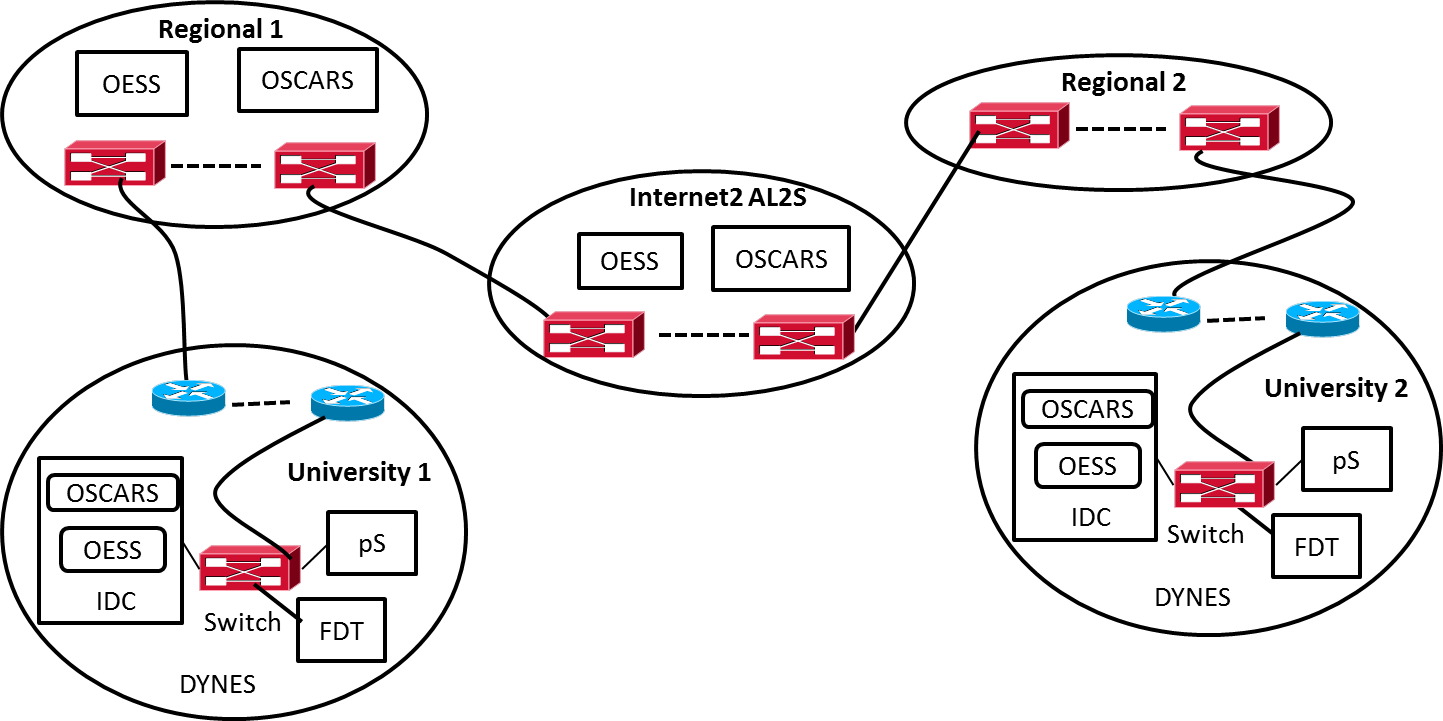
\includegraphics[width=0.7\textwidth]{figures/multi-domain-network.png}
\caption{An illustration of our multi-domain dynamic L2 path service deployment; Fast Data Transfer (FDT) server; Inter-Domain Controller (IDC); perfSONAR (pS) host; Open Exchange Software Suite (OESS); On-Demand Secure Circuits and Advance Reservation System (OSCARS); Advanced Layer 2 Service (AL2S)}
\label{fig:network}
\end{figure}

Each university
campus DYNES equipment, as shown in Fig.~\ref{fig:network},
consists of three hosts: Fast Data Transfer (FDT) server, Inter-Domain Controller (IDC) host, perfSONAR (pS) \cite{perfSONAR} host,
and one Ethernet switch (which is OpenFlow enabled in some sites). The FDT server runs data-transfer applications, the IDC host runs the control-plane software (OSCARS, and OESS at sites with an OpenFlow-enabled switch), and the pS host runs active-measurement tools for monitoring network performance.

Some regional RENs such as Regional 1 in Fig.~\ref{fig:network}
run OSCARS and OESS controllers to offer dynamic
L2 path service while others such as Regional 2 in
Fig.~\ref{fig:network} offer only static L2 path service and
hence do not deploy OESS and OSCARS.
As can be expected with the roll-out of a new networking
service, organizations will slowly deploy the service
one-at-a-time. Static L2 path service is available from most RENs
and university campus networks, and can be used to bridge gaps in the
dynamic L2 service offering.

Internet2's Advanced Layer-2 Service (AL2S) network has 39 OpenFlow-enabled
Ethernet switches, as shown in Fig~\ref{fig:AL2S}, and is operated in L2 Virtual LAN (VLAN) mode.
AL2S delivers a strategic advantage for leaders in research and education (R$\&$E) by providing effective and efficient wide area 100 gigabit Ethernet technology. AL2S allows users to create their own VLANs on the Internet2 AL2S backbone. Static or Dynamic, point-to-point or multipoint, intra-domain or inter-domain, AL2S puts control of the backbone VLANs into the users' hands for the creation of purpose-built private circuits using infrastructure already in place. AL2S is available to 279 higher education institutions include Univeristy of Virginia. AL2S uses OESS for controlling the OpenFlow switches, and OSCARS for inter-domain L2 paths.
\begin{figure*}[htbp!]
\centering 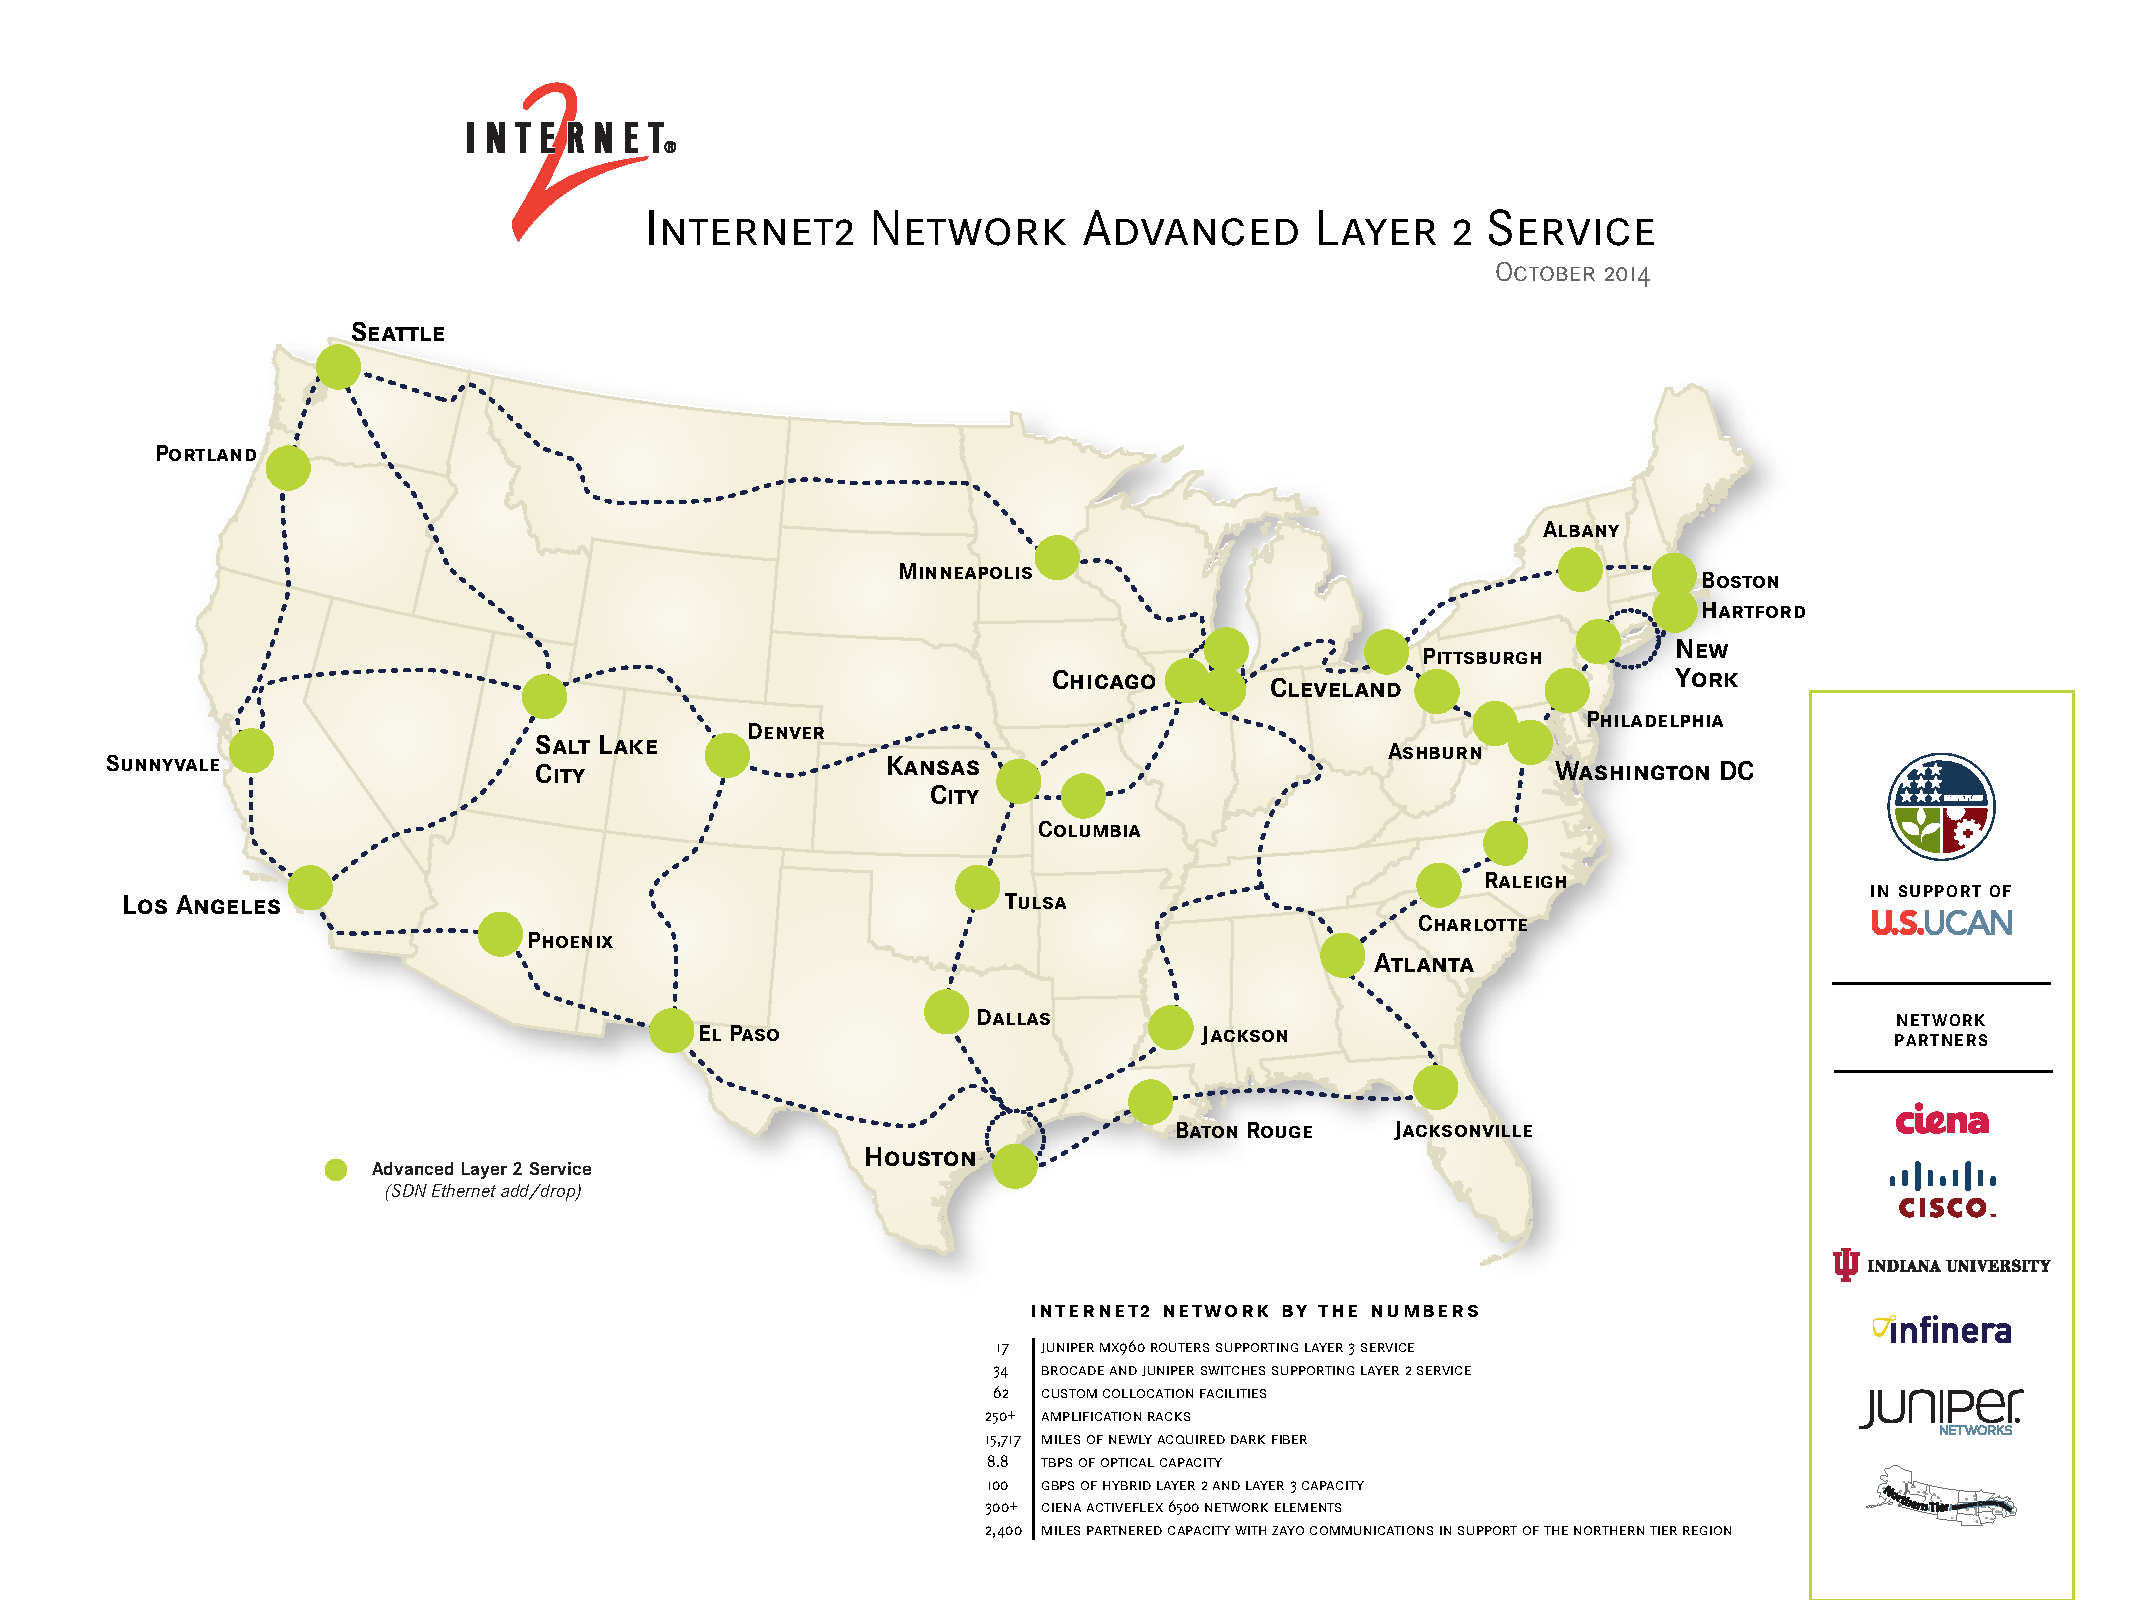
\includegraphics[width=0.80\textwidth]{figures/AL2S.pdf}
\caption{Internet2 Advanced Layer 2 Service (AL2S) Network}
\label{fig:AL2S}
\end{figure*}

We \emph{first} describe how the
DYNES equipment was configured at each site.
\emph{Next}, we describe the actions needed within campuses between the
location of the DYNES equipment and the campus edge. \emph{Finally},
we describe the actions required from regional RENs
that did not deploy this dynamic L2 path service.

\textbf{Step 1.} At each DYNES site, we logged in to the OpenFlow
enabled switch, configured the IP address of the IDC host
on which the OESS (OpenFlow controller) is being run, and
added the set of ports to be controlled by the OESS into
the switch's OpenFlow instance (only one instance is used).
The OpenFlow switch models used by the DYNES project
support \emph{hybrid-switch} mode in which OpenFlow controlled
and traditionally configured ports can co-exist on the switch.
However, these switches do not support \emph{hybrid-port} mode in
which each individual port can be controlled by both the
OpenFlow controller and traditional configuration methods.

The next set of operations at each DYNES site consisted of
(i) initiating OESS and OSCARS on the IDC host, (ii) providing the OESS with the switch's control-port IP address,
and (iii) configuring OESS and OSCARS through their Web
UIs. Specifically, the OESS UI is used to set the remote-link
information for the data-plane port of the peering network.
For example, the UVA DYNES switch port 1 is connected
to say port 1 of a UVA campus router. A static VLAN was
configured from port 1 of this UVA campus router through
the other UVA campus routers, and through the regional
REN (MARIA) routers to the MARIA router port that is
connected to port et-3/0/0.0 on the Internet2 AL2S switch
in Ashburn, VA. This static VLAN serves as the remote
link between UVA DYNES network and Internet2 AL2S.
Information about this remote link is entered into the UVA
DYNES OESS to identify the peering domain, node, and
port. The counterpart action was performed at Internet2's
OESS for the UVA DYNES switch remote link. This remote-link information was provided manually to Internet2. The
OESS UI is also used to configure the set of allowed VLANs
on each port of the DYNES switch.

UVA DYNES OSCARS needed to be configured with a server certificate, and the certificate owner and issuer information needed to be manually communicated to Internet2's administrator for configuration of Internet2's AL2S OSCARS. These certificates are used in the authentication
process for inter-domain L2 path requests.

\textbf{Step 2.} Most of the involved campus networks and regional
RENs support static L2 path services. This allowed us to request and obtain provisioned L2 paths with a specified set of
VLAN IDs from campus network administrators. These L2
paths cut across the campus switches/routers between the
DYNES equipment and the campus edge router. Having the
capability to establish static L2 paths allows for a gradual
introduction of OpenFlow switches under OESS control into
campus networks.

\textbf{Step 3.} Similarly, we contacted regional REN administrators to obtain static L2 paths with specified VLAN IDs
across their networks to Internet2. Again this capability of using static L2 paths allows for a gradual addition of
dynamic L2 path service by different regionals at different
times, and yet support dynamically created end-to-end L2
paths.

The above experience shows the various steps required to
configure OSCARS and OESS in each organization that is
ready to support dynamic L2 service, as well as the feasibility of using static L2 paths through networks whose organizations are not as-yet ready for the dynamic service.

\subsection{Path/VLAN provisioning through switches}
\label{sec:multidomain-SDN-path-provisioning}

This section describes the process of establishing a new VLAN via the OESS UI \cite{OESS}. We use the term ``path'' if the VLAN has just two
endpoints, and the term ``multipoint VLAN'' if there are multiple endpoints.

After user authentication in the OESS UI through the login process, the OSCARS IDC workgroup should
be selected. Then in the Actions tab, the user should select the \texttt{Create a New VLAN} option. The system then guides the user through a 6-step procedure to provision a VLAN.

\paragraph{Step 1:  Basic characteristics}
Fig.~\ref{fig:oessbasic} shows a screenshot of the first step for a local circuit, and Fig.~\ref{fig:oessbasic-interdomain} shows a screenshot of the first step for an inter-domain circuit.
In both cases, the user should enter a human-readable name for the VLAN being created in the
\texttt{Description} field. For inter-domain paths, the user is offered the option of specifying
bandwidth for the circuit (see Fig.~\ref{fig:oessbasic-interdomain}), but not for intra-domain (local) paths (see Fig.~\ref{fig:oessbasic}).
 If the user wants a failed VLAN that had been automatically routed to a backup path to be restored to the primary path, the \texttt{Restore to Primary} field should be enabled. If the VLAN can stay routed on the backup path, this field can left in the \texttt{Off} state. The \texttt{Multipoint Static MAC Routing} field allows a user to associate a destination MAC addresses with each endpoint of a multipoint VLAN. Packets destined to such a configured MAC address will be forwarded to only the corresponding endpoint rather than to all endpoints as would happen if this feature was left disabled, or for packets with destination MAC addresses that were not attached to any endpoints of the multipoint VLAN.
 This field is only offered for local (intra-domain) paths (see Fig.~\ref{fig:oessbasic}), and
 not for inter-domain paths (see Fig.~\ref{fig:oessbasic-interdomain}). The \texttt{Type of Circuit} field should be set by the user to \texttt{Local}, if the VLAN traverses the single domain controlled by the particular OESS whose UI is being accessed. If the VLAN will
need to traverse multiple domains, the user should select the \texttt{Interdomain} option. This
option will cause the OESS to obtain all accessible endpoints from the
OSCARS topology service as described in Section~\ref{sec:OESS}, and load these into the UI in the next step for endpoint selection.

\begin{figure}[htb!]
\centering
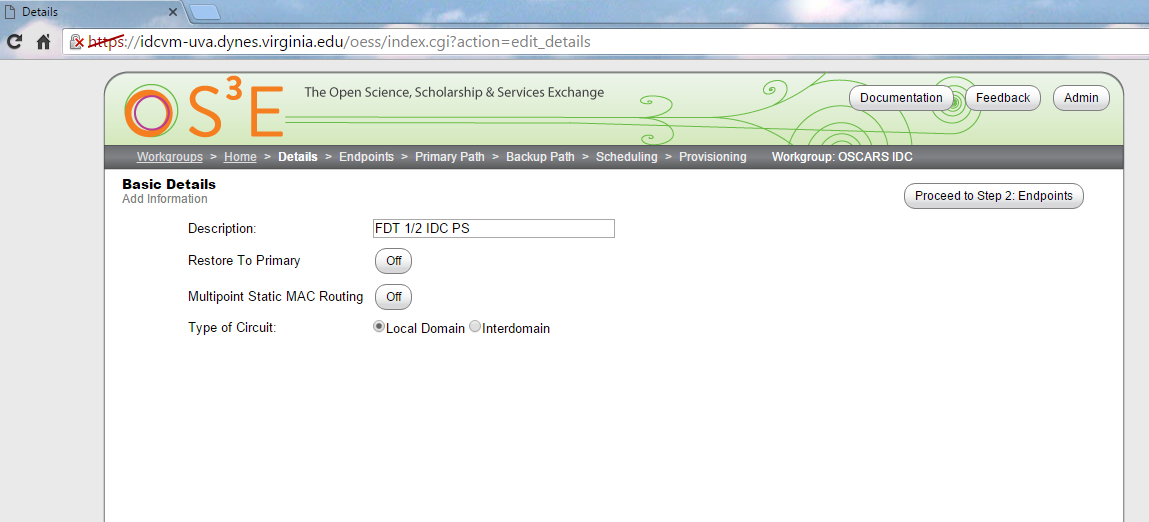
\includegraphics[width=0.8\textwidth]{figures/oess-basic.png}
\caption{OESS UI Step 1: Choose basic characteristics for an intra-domain path}
\label{fig:oessbasic}
\end{figure}

\begin{figure}[htb!]
\centering
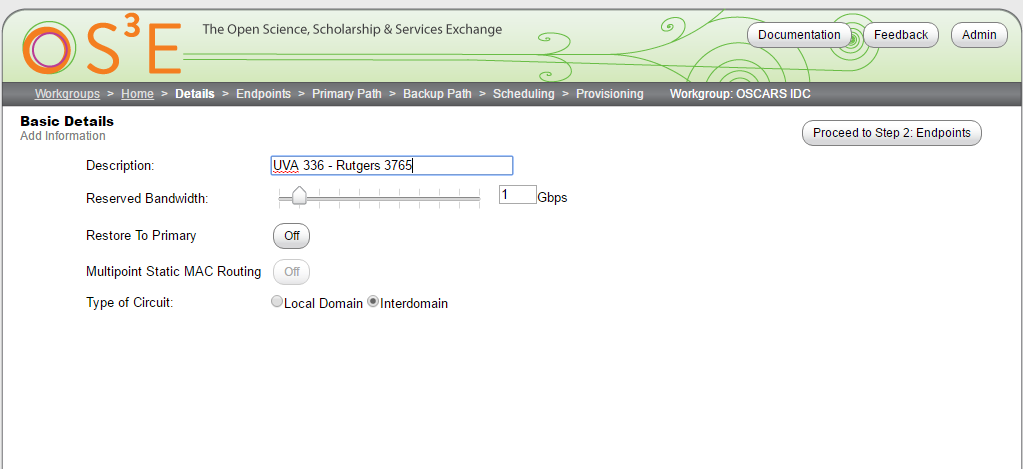
\includegraphics[width=0.8\textwidth]{figures/oess-basic2.png}
\caption{OESS UI Step 1: Choose basic characteristics for an inter-domain path}
\label{fig:oessbasic-interdomain}
\end{figure}



\paragraph{Step 2: Endpoints and VLAN IDs}
Fig.~\ref{fig:oesspoints} shows Step 2, in which the user selects the endpoints of the VLAN.
For each endpoint, the user needs to provide a corresponding VLAN ID. The user starts by clicking on the dot in the map displayed on the screen. In this example, the single dot represents the UVA DYNES switch. Since the \texttt{Type of Circuit} field was set to \texttt{Local} in Step 1,
OESS displays just the seven endpoints of the UVA DYNES network (on the bottom right corner). Specifically, these endpoints are ports on the single UVA DYNES switch served by the OESS being used for this provisioning process. When the user clicks on a port that should be an endpoint in the VLAN, OESS displays a window in which the user is required to provide a specific VLAN ID. Each workgroup is provided rights to use specific VLAN IDs for each endpoint. Hence
authorization is run by OESS allows before a particular VLAN ID is used for provisioning. In this
example, the user has selected four interfaces, specifically ports 0/19, 0/24, 0/22, and 0/20,
of the UVA DYNE switch,
and hence these interfaces are displayed under \texttt{Endpoints} in the main part of the screen.
The user has selected the same VLAN ID 332 for all four endpoints.
\begin{figure}[htb!]
\centering
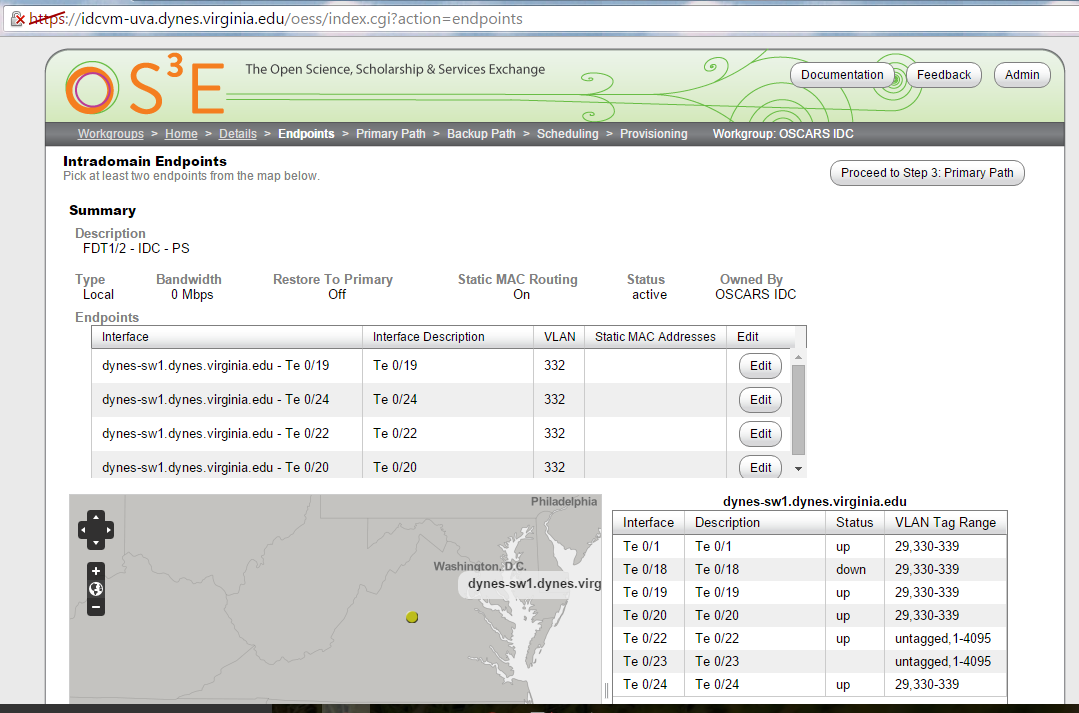
\includegraphics[width=0.8\textwidth]{figures/oess-points.png}
\caption{OESS UI Step 2: Selection of endpoints and VLAN IDs}
\label{fig:oesspoints}
\end{figure}

\paragraph{Step 3: Select primary path}
Fig.~\ref{fig:oessprimary} shows the OESS UI screenshot for Step 3 in which the user can select a path or ask OESS to suggest the shortest path. If a user is not particular about the selected path, users can click on the\texttt{ Suggest Shortest Path} button, and OESS will find the shortest path between the selected endpoints. Alternatively, a users can click on links to add or remove them from a path. The path must connect the endpoints and must not have any loops. For the example show, since the three interfaces are on the same UVA DYNES switch, there is only one possible multipoint VLAN.
\begin{figure}[htb!]
\centering
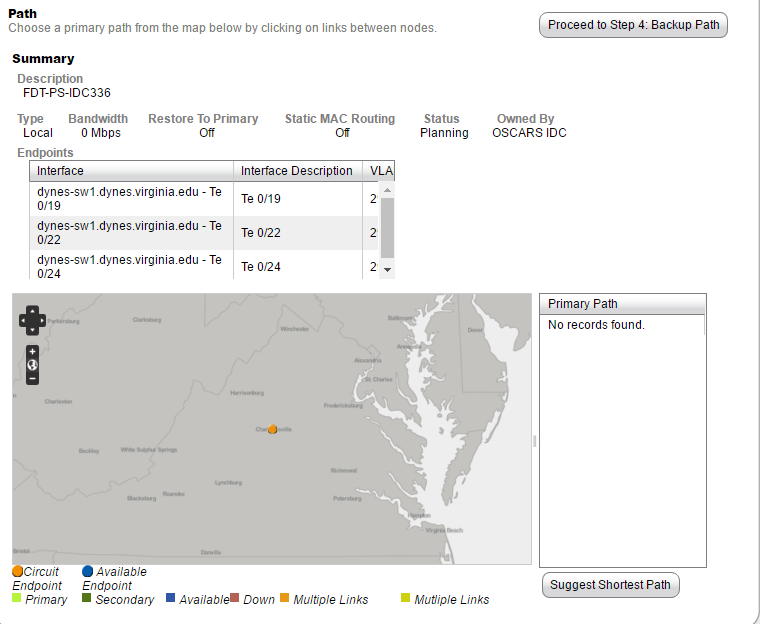
\includegraphics[width=0.8\textwidth]{figures/oess-primary.png}
\caption{OESS UI Step 3: Primary path selection}
\label{fig:oessprimary}
\end{figure}

\textbf{Step 4: Select backup path}
In Step 4, a user can select a backup path for automatic switch-over from the primary path in case of
failures. If the user clicks on the \texttt{Suggest Shortest Path} button, the OESS will attempt to find an path that has minimal overlap with the primary path.  Selection of a backup path is optional. Fig.~\ref{fig:oessbackup} shows a screenshot of the OESS UI Step 4.
\begin{figure}[htb!]
\centering
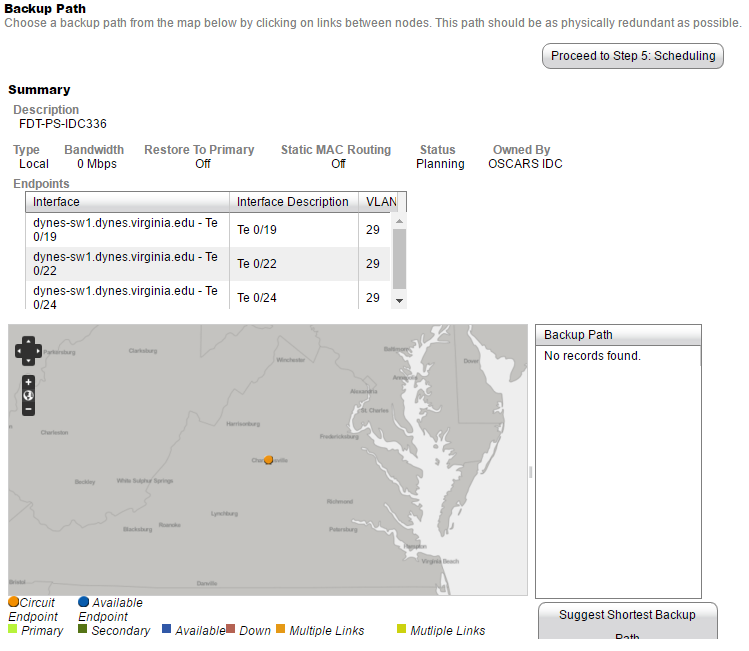
\includegraphics[width=0.8\textwidth]{figures/oess-backup.png}
\caption{OESS UI Step 4: Backup path selection}
\label{fig:oessbackup}
\end{figure}

\textbf{Step 5: Scheduling}
\begin{figure}[htb!]
\centering
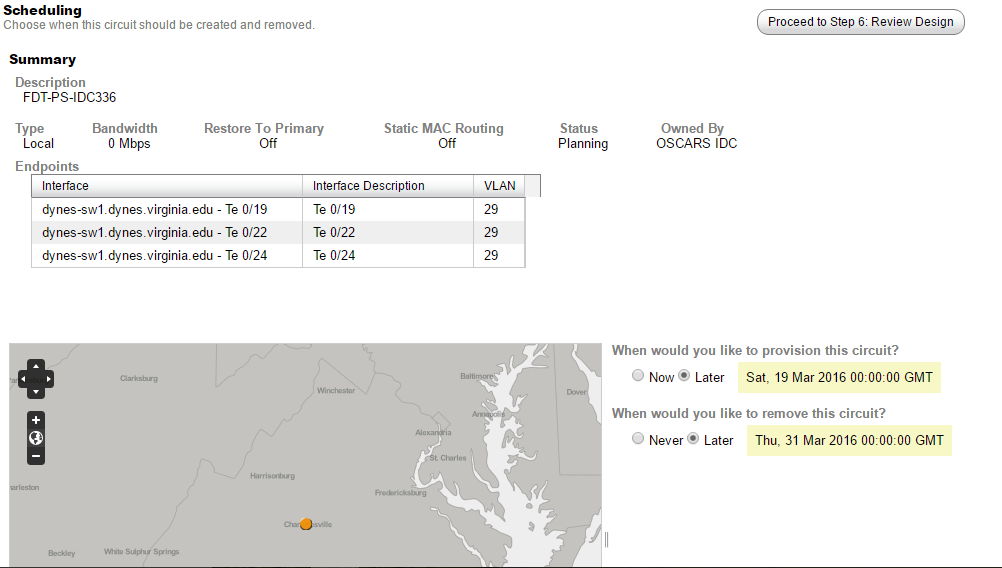
\includegraphics[width=0.8\textwidth]{figures/oess-schedule.png}
\caption{OESS UI Step 5: Circuit scheduling}
\label{fig:oessschedule}
\end{figure}
Fig.~\ref{fig:oessschedule} shows a screenshot of the OESS UI Step 5, in which a user can specify
a start time and release time for the circuit. In the example shown, the user
has requested a later
start time (not ``now''), and has specified a particular future date when the circuit should be released.

\paragraph{Step 6: Review design and submit circuit request}
Users are given an opportunity to review the design before selecting
the \texttt{Submit Circuit Request}.
Fig.~\ref{fig:oessreview} shows the corresponding OESS UI screenshot.
\begin{figure}[htb!]
\centering
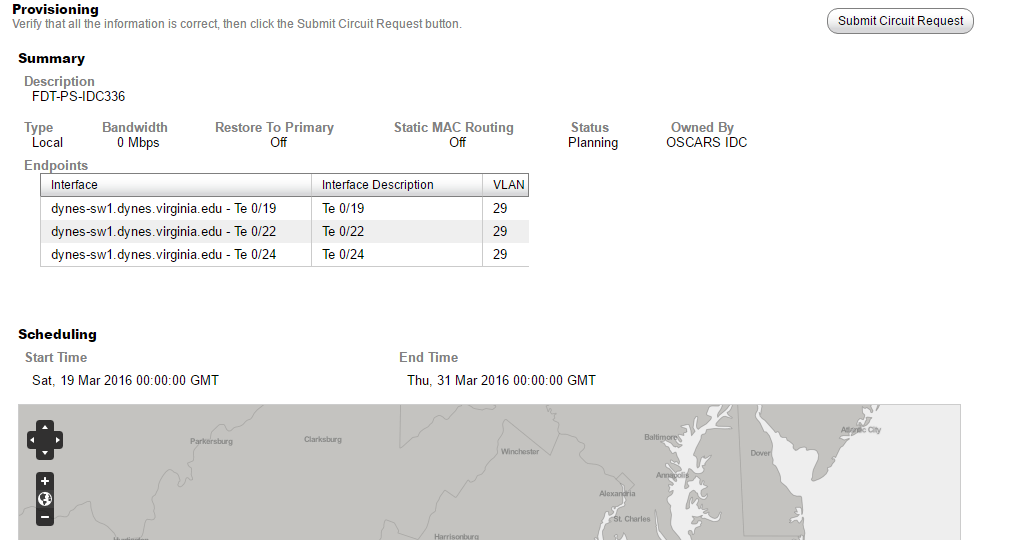
\includegraphics[width=0.8\textwidth]{figures/oess-review.png}
\caption{OESS UI Step 6: Review design}
\label{fig:oessreview}
\end{figure}

If the OESS is successful in setting up the circuit between the selected endpoints
at the specified rate, in the time interval specified in Step 4, a success message
is displayed to the user through the UI. If not, a failure message is displayed.
One of the drawbacks of the current software is that failure messages do
not offer a cause for the failure.

\subsection{Path Configuration at Hosts}
\label{sec:multidomain-SDN-FDT-access}
Three steps are required to configure the FDT hosts at the
ends of an L2 path: (i) a VLAN with the appropriate VLAN
ID is configured on the FDT NIC that is connected to the
DYNES switch, (ii) IP addresses on the same subnet are
assigned to the VLANs configured at the two FDT hosts,
and (iii) the traffic control (\texttt{tc}) Linux utility is configured
to rate limit outgoing traffic to the L2-path rate used in the
path-reservation phase.
\begin{figure}
\centering
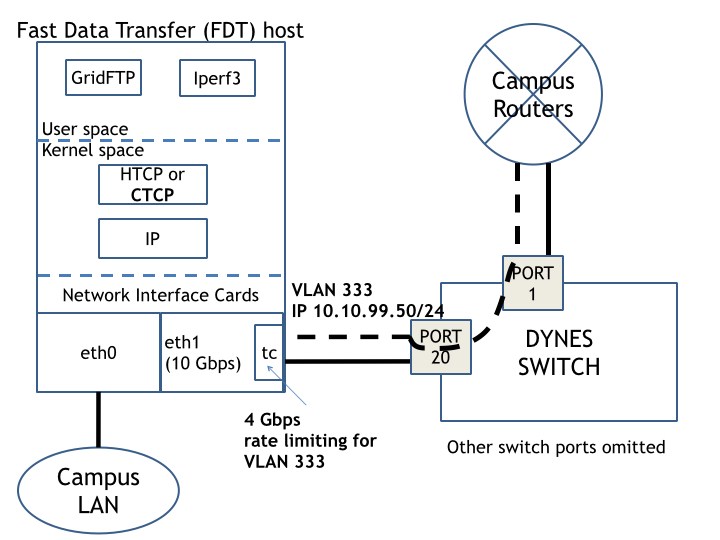
\includegraphics[width=0.6\textwidth]{figures/uvadynes.png}
\caption{Configuring the Fast Data Transfer (FDT) host for the L2 path}
\label{fig:uvadynes}
\end{figure}

Fig.~\ref{fig:uvadynes} illustrates the UVA DYNES data-plane with a configured VLAN for the end-to-end L2 path to the IU FDT.
However before discussing the details of Fig.~\ref{fig:uvadynes}, recall the example end-to-end L2 path described in Fig.~\ref{fig:AL2S} between
port 19 of the DYNES switch in the University 1 network,
and port 20 of the DYNES switch in the University 2 network of Fig.~\ref{fig:AL2S}. While the endpoints specified in the request
to the OESS are the two switch ports, the L2 path essentially
extends between the FDTs at University 1 and University 2
as the specified switch ports are connected to the FDTs.

Therefore, the VLAN ID used on the interface from the FDT
to the DYNES switch in the request to the OESS needs to
now be configured in the FDT. In the example shown in
Fig.~\ref{fig:uvadynes}, the VLAN ID used in the request to the OESS for
port 20 of the UVA DYNES switch for the L2 path to the
IU FDT was 333. Now, using the Linux \texttt{vconfig} command
in the UVA FDT, the user or application needs to configure
VLAN 333 on the \texttt{eth1} NIC, which is the one connected to
port 20 of the DYNES switch.

The second step that needs to be executed on the FDT is a
configuration of an IP address associated with the newly created VLAN. For this purpose the Linux \texttt{ifconfig} command
is used. Fig.~\ref{fig:uvadynes}shows that private IP address 10.10.99.50
is assigned to VLAN 333 on \texttt{eth1}. IP packets sent out
with source IP address equal to 10.10.99.50 will be carried
in tagged Ethernet frame headers with VLAN ID set to 333.

Fig.~\ref{fig:uvadynes} also shows that the FDT host has another NIC, \texttt{eth0}
for connectivity to the campus LAN. This interface for logging into the FDT remotely using an ssh client.

The reason for needing to configure IP on the VLAN is to allow for the usage of existing applications, such as GridFTP
and \texttt{nuttcp}, and transport-layer protocols such as HTCP \cite{HTCP}
as illustrated inside the FDT in Fig.~\ref{fig:uvadynes}. Packets sent on the
end-to-end L2 path are not subject to L3 (IP) header based
packet forwarding because all switches on the path have
been provisioned to execute packet forwarding based on the
VLAN ID. IP headers are nevertheless included/extracted at
the FDT servers because of the applications' use of TCP/IP
sockets.

Furthermore, the private IP addresses configured for the
FDT VLANs at the two ends need to belong to the same
subnet to avoid having to add destination-specific routes to
the IP-routing table in the FDTs. For this L2 path, the
VLAN ID used on the port of the IU DYNES switch was
2399 and the IP address assigned to VLAN 2399 on the
Ethernet NIC in the IU FDT host was 10.10.99.40.

In our usage of these L2 paths,
we manually executed these VLAN and IP address configuration commands at the FDT hosts, having procured privileged access for the execution of these commands. However, for general-purpose use of L2 path-based networking, applications should be integrated (through shell scripts or with
modifications) with a signaling-client module that issues requests for paths to OESS, handles responses, and additionally configures VLANs and IP addresses at the FDTs. Further, an end-to-end session protocol is required to exchange
subnet identifier/mask information to ensure that the private IP addresses assigned to the VLANs at the two end
FDTs match. Since the FDT and IDC servers have multiple Ethernet interfaces, one of which is connected to the campus IP-routed
infrastructure, e.g., \texttt{eth0} in the FDT shown in Fig.~\ref{fig:uvadynes}, L3 IP
service is used for all signaling messages.

Finally, Fig.~\ref{fig:uvadynes} shows that the Linux \texttt{tc} utility is used in the
FDT host to limit the rate at which the 10Gbps \texttt{eth1} NIC
transmits frames. The example VLAN shown was created
with a 3 Gbps rate request; therefore, \texttt{tc} would have been
configured to rate limit VLAN-333 Ethernet frames to 3
Gbps.

\subsection{Data plane Experiments}
\label{sec:multidomain-SDN-data-plane-expts}

This section describes the methodology used to test a newly provisioned VLAN.
It not only verifies that the VLAN has been successfully provisioned across the network(s), 
but also verifies the configuration actions at the end hosts.
\begin{figure}[htb!]
\centering
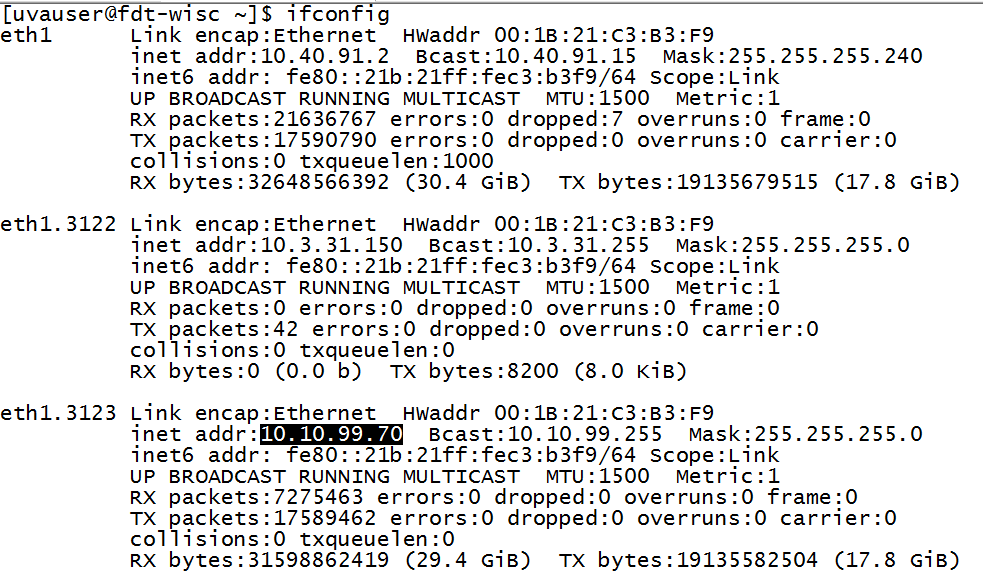
\includegraphics[width=0.8\textwidth]{figures/ifconfig.png}
\caption{Linux utility \texttt{ifconfig}}
\label{fig:ifconfig}
\end{figure}
An interdomain circuit was configured from the FDT at UWisc to the FDT at UVA. The VLAN ID
at the UWisc FDT was 3123, and at the UVA FDT, it was 336. The IP addresses/subnet masks 10.10.99.70/24 and 10.10.99.50/24 were assigned to the UWisc FDT VLAN and UVA FDT VLAN,
respectively.

Before running an end-to-end data-plane test, the Linux utility \texttt{ifconfig} was used to check the configuration of the VLANs at both ends. Fig.~\ref{fig:ifconfig} shows the UWisc interface \texttt{eth1} was configured with a VLAN with ID 3123, and this VLAN was
 assigned IP address 10.10.99.70 with subnet mask /24.

Next, the \texttt{ping} command was executed to test the reachability across this newly configured VLAN path from UWisc FDT to UVA FDT.
 Fig.~\ref{fig:ping} shows that the UVA FDT VLAN was reachable from the UWisc FDT,
 as the latter receives a reply to the ping command sent to IP address 10.10.99.50, which is
 the address that was assigned to VLAN 336 at the UVA FDT interface. Success of this
\texttt{ping} execution verifies that the L2 path was successfully setup across all five domains,
UWisc, CIC OmniPoP (regional REN for UWisc), Internet2 AL2S, MARIA (regional REN for UVA),
and UVA. Further it attests to the successful configuration of the two end hosts.

\begin{figure}[htb!]
\centering
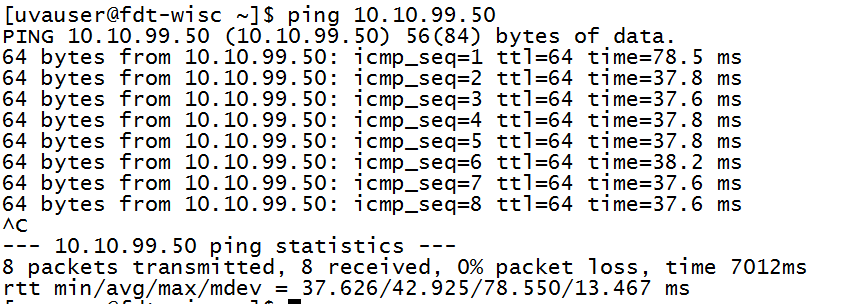
\includegraphics[width=0.8\textwidth]{figures/ping.png}
\caption{Linux utility ping}
\label{fig:ping}
\end{figure}



\section{Insights Gained}
\label{sec:insights}

Section~\ref{sec:config-ovhd} describes the configuration
overhead required to run this dynamic L2 path service, and addresses
the question of scalability.
Section~\ref{sec:ckt-provisioning} describes
our experience as users of OSCARS and OESS in configuring
inter-domain L2 paths.
Finally, Section~\ref{sec:other-challenges} describes
other challenges we faced in the course of this deployment.

\subsection{Configuration Overhead and Scalability}
\label{sec:config-ovhd}
A number of administrator
actions are required to configure the OpenFlow switches, OESS and OSCARS. The
larger the number of such required actions, the greater the
potential for administrator errors.
Effort is required to reduce the number of required administrator
actions wherever possible.

To achieve a global-scale dynamic L2 path-service deployment,
the current solution for making available endpoint information
through the OESS Web user interface to allow for user selection of path endpoints
needs
to be changed. A potential solution for allowing users to find the
endpoint identifiers for hosts that support dynamic L2 path service is
to incorporate this service into the widely deployed DNS system. If a user
has the domain name of a host that supports dynamic L2 path service, a new DNS
resource record could provide the translation of this name to the endpoint
identifier required by OESS and OSCARS.

Finally, the scalability and usability of the pS Topology Service should be assessed.
As described in Section~\ref{sec:control-plane}, the OSCARS topology service
pushes the topology of a domain to the pS Topology Service, allowing OSCARS
in other domains to request topology information when needed. While this open
topology sharing approach works in the REN community, it is not suitable
for commercial providers. Contrast this approach to the more practical Border Gateway Protocol solution of sharing only address reachability across domains.
Therefore, this part of the OSCARS design needs to be revisited.


\subsection{Path Provisioning and Testing}
\label{sec:ckt-provisioning}

The OESS and OSCARS software systems were relatively stable and their Web user interfaces were fairly easy to navigate. In general, these controllers are
robust and allowed us to set up and tear down inter-domain paths dynamically.
However, three aspects need improvement: error reporting, path setup delay,
and path failure debugging.

The error reporting functionality of OSCARS needs to be enhanced. Path setup failures
occur due to a lack of bandwidth, unavailability of a requested VLAN ID, or due to an expired certificate. In all these cases, while OSCARS reports a failed setup attempt,
the error messages are cryptic and do not offer users a decipherable reason for the failure.

The second issue relates to setup delay and the OSCARS approach of handling only one path setup at a time.
In particular, a failed path setup attempt causes OSCARS to wait for a user-configured timeout interval, which is currently set to 15 min. While this solution is sufficient for low call arrival rates, a programmatic test with multiple path setup-and-release attempts experienced excessive delays.

Finally, the lack of L2 connectivity tools comparable to L3 tools such as \texttt{ping} and \texttt{traceroute} made it difficult to identify the domain in which the L2 connectivity
was broken.
We used three methods to debug such connectivity issues. First, we had campus and regional REN administrators configure a specified private IP address to a specified VLAN on the port of their domain's edge router that is connected to the next domain (toward Internet2). This allowed us to use L3 tools
to verify that static VLANs across each domain were operational. Second, we used observatory hosts located at Internet2 PoPs whose ports (with specified VLANs) were made available by Internet2 to DYNES users for L2 path testing. This allowed us to create dynamic L2 paths between each campus DYNES switch and an observatory host's Internet2 router port for single campus-and-regional segment testing. Finally, we used GRNOC's routerproxy tool \cite{routerproxy} to observe packet counts at router ports while sending data between campus FDTs on configured VLANs to localize problems. These methods are rudimentary and suitable for the REN community,
but better methods leveraging OpenFlow features need to be developed.

\subsection{Other Challenges}
\label{sec:other-challenges}
In the course of one year, we experienced software upgrades to OSCARS,
X.509 certificate expirations, and even network connectivity changes (regional networks
were moved to AL2S from ION for their Internet2 access). Each of
these changes required corresponding administrative actions, sometimes in several
DYNES sites and Internet2. For example, OSCARS server peerings and topology
files had to be updated
when a regional moved its access link from Internet2's Interoperable On-demand Network (ION) to AL2S.






\section{Multi-point VLAN}
\label{sec:mdvlan}

\subsection{Control Plane Setup}
\label{sec:controlplanefinal}
A Multipoint VLAN can be created by OESS. However, the multipoint VLAN feature in OESS is only supported for intra-domain circuit. For provisioning a inter-domain multipoint VLAN, two steps are required. First, we created a local domain multipoint VLAN in AL2S OESS where multiple switches in different regions are selected as the endpoints. Second, we provisioned a point-to-point VLAN by OESS from the endpoint in each site to its regional network which is connected to AL2S switches. Fig.~\ref{fig:campus-regional} presents the campus-regional VLAN provisioning from UVA FDT to AL2S Ashburn switch.
\begin{figure}[htb!]
\centering
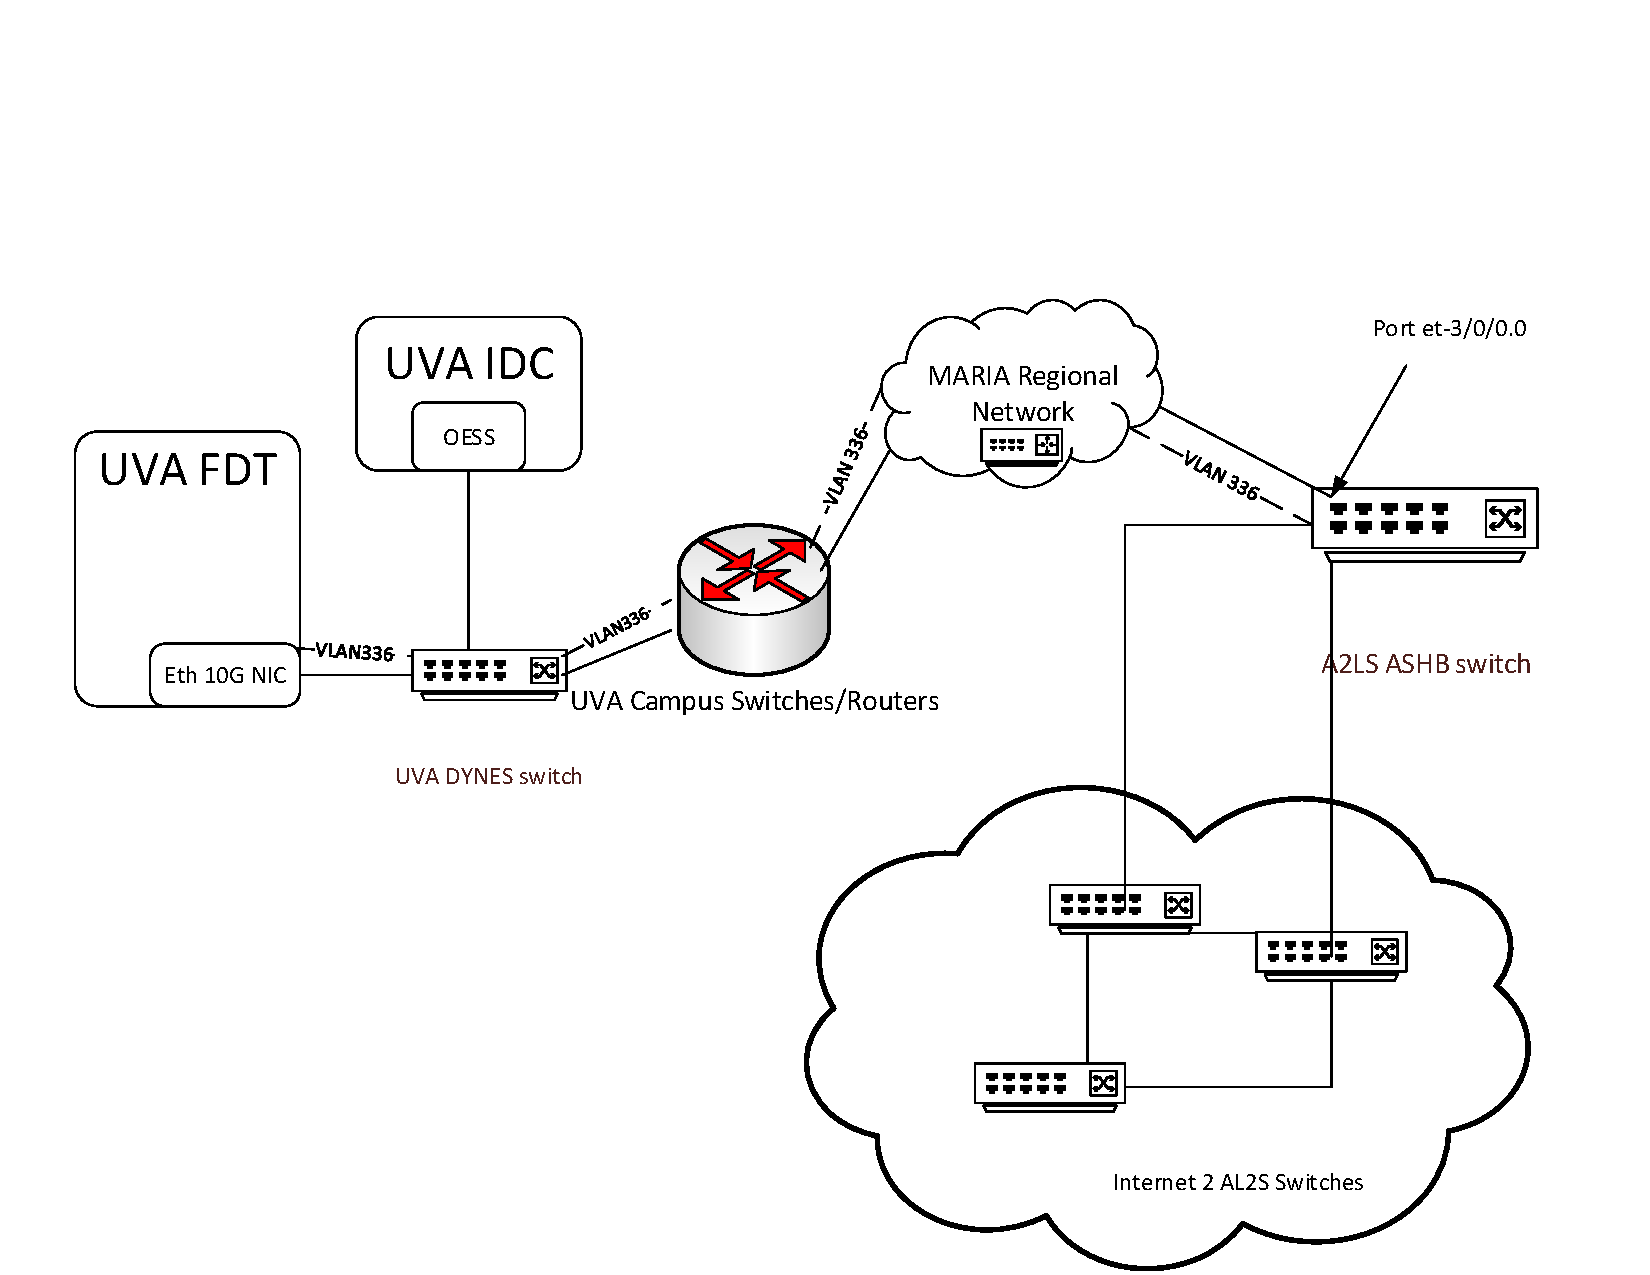
\includegraphics[width=0.8\textwidth]{figures/UVA-ASHB.pdf}
\caption{UVA DYNES - UVA campus – MARIA- ASHB}
\label{fig:campus-regional}
\end{figure}
Fig.~\ref{fig:wanmulticast} shows a inter-domain multipoint VLAN setup among University of Virginia (UVA), Indiana University (IU), Mid-Atlantic Crossroads (MAX). AL2S OESS created a multipoint VLAN where the AL2S switches conducted the VLAN translation for packets came from each site. When the AL2S switch received packets with VLAN ID 336 from UVA, it made two copies of packets and set two different VLAN ID 2399, 1830, and forward the packets to IU and MAX.

Fig.~\ref{fig:oessal2s} shows the endpoints and VLAN tags selection of a multipoint inter-domain path among UVA, MAX, and IU. Different VLAN tags are selected for the corresponding interfaces in each site.

\begin{figure}[htb!]
\centering
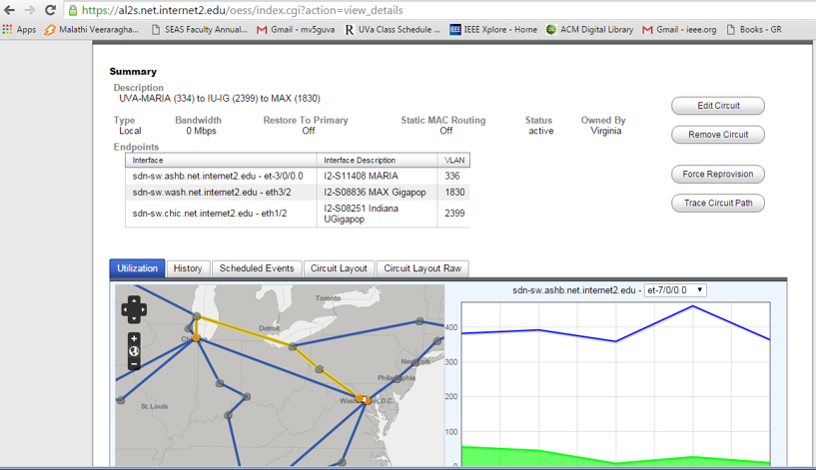
\includegraphics[width=0.8\textwidth]{figures/oess-AL2S.png}
\caption{AL2S OESS: Endpoints and VLAN selection}
\label{fig:oessal2s}
\end{figure}

\begin{figure}[htb!]
\centering
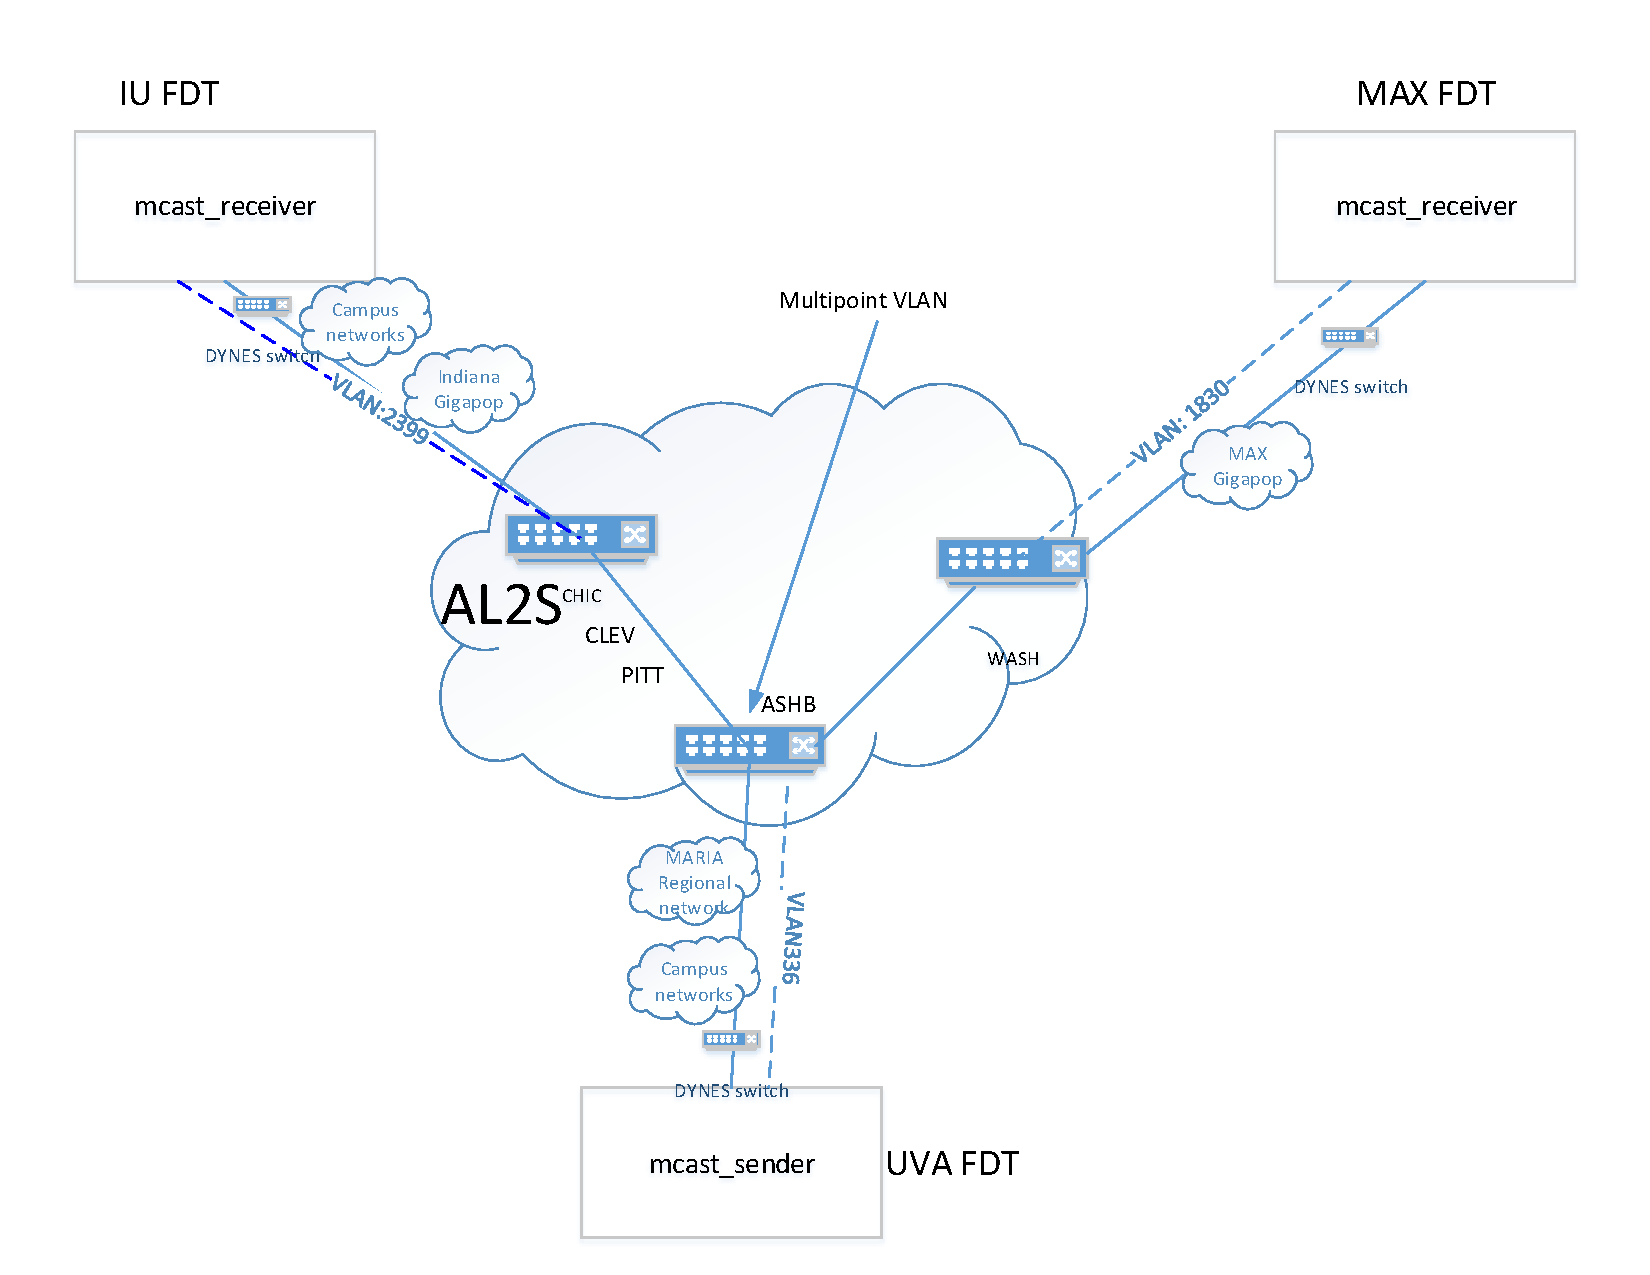
\includegraphics[width=0.8\textwidth]{figures/AL2S-mcast.pdf}
\caption{AL2S inter-domain multipoint circuit experiment}
\label{fig:wanmulticast}
\end{figure}




\subsection{Data Plane Experiments}
\paragraph{Experimental Setup}
Dynamic Network System (DYNES) \cite{1742-6596-396-4-042065}, an NSF funded nationwide cyber-instrument spanning about 40 US universities and 14 Internet2 connectors. A collaborative team including Internet2, Caltech, University of Michigan, and Vanderbilt University worked with regional networks and campuses to support large, long-distance scientific data flows and scientific community. DYNES testbed was used to run all the OpenFlow multicast experiments. Users are offered OESS Web GUI to provision dynamic multipoint layer-2 circuits. For my experiments, we setup a multipoint VLAN via AL2S OESS among five DYNES sites at (i) University of Virginia (UVA), Charlottesville, VA, (ii) Indiana University (IU), Indianapolis, IN, (iii) Mid-Atlantic Crossroads (MAX), College Park, MD, (iv) Rutgers University (Rutgers), New Brunswick, NJ (v) University of Wisconsin–Madison (UWisc), Madison, WI. Each DYNES FDT host has two Intel Xeon
E5620 four-core processors (for a total of eight cores) and
24 GiB of RAM.

The software used in my experiments consists of: (i) IP multicast test program for sending and receiving multicast traffic.  (ii) Linux utility \texttt{vconfig} to configure VLAN tag for interface  (iii) Linux \texttt{ifconfig} to configure IP address and subnet mask for VLAN interface. (iv) Linux utility \texttt{ping} to test the reachability of a host. (v) Linux utility \texttt{tcpdump} to capture packet information of the multicast traffic packet with VLAN tag and multicast IP and MAC address.

\paragraph{Experiments Execution and Results}
First, we describe the local multipoint experiments workflow. Next, we present the inter-domain multipoint experiments results and our debugging experience.

%%%%oess, fdt several sentences, mcast program

First, A multicast test was conducted within a intra-domain multipoint topology showed in Fig.~\ref{fig:oesspoints}. After the multipoint circuit was created by OESS, several corresponding flow entries would be inserted into the flow table of UVA DYNES switch. As Fig.~\ref{fig:flowtable} shows, when the switch receives a packet from port Te 0/19 with VLAN tag 332, it will take the actions which set the VLAN id 332 and forward the packet to port Te 0/20, Te 0/22, Te 0/24. After the OpenFlow multipoint VLAN was set up, we configured VLAN interfaces at each hosts. The hosts configuration process is described in Section~\ref{sec:multidomain-SDN-FDT-access}. All the IP addresses of the hosts need to be private and within a same subnet. Next, we used \texttt{ping} utility to test the VLAN setup.

\begin{figure}[htb!]
\centering
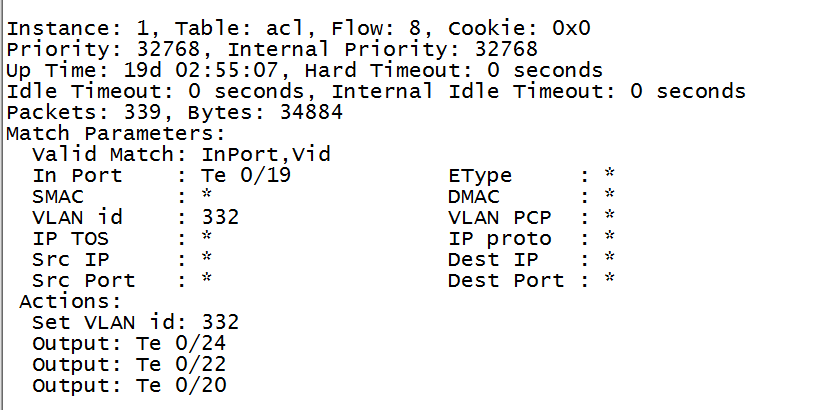
\includegraphics[width=0.8\textwidth]{figures/flow-table.png}
\caption{OpenFlow flow table entry of UVA DYNES switch}
\label{fig:flowtable}
\end{figure}

Second, a IP multicast program was run to test the multipoint OpenFlow path. This IP multicast program is used for multicast testing
over wide-area network. It includes a multicast sender and a multicast receiver,
which can be compiled and executed on different Linux-based hosts over the wide-area environment.
We executed the multicast sender in UVA FDT and multicast receivers in the other two local DYNES hosts(IDC and pS).
As Fig.~\ref{fig:localmulticast} shows, the interfaces unicast IP addresses for sending or receiving the multicast should be specified as the first argument of the program. The reason for specifying the unicast IP address of the interface is so that multicast packets are sent to the interface with this IP address. This unicast IP address (10.30.32.20) identifies the interface. All multicast traffic generated in this socket will be output from the interface chosen. The multicast group IP address and port are the last two arguments. A UDP datagram socket is created using this multicast group IP address and port. In the code, after the UDP socket is created with the multicast IP address 233.0.225.123 and port 8888, \texttt{setsockopt} is called to set two parameters: interface and TTL.

\begin{figure}[htb!]
\centering
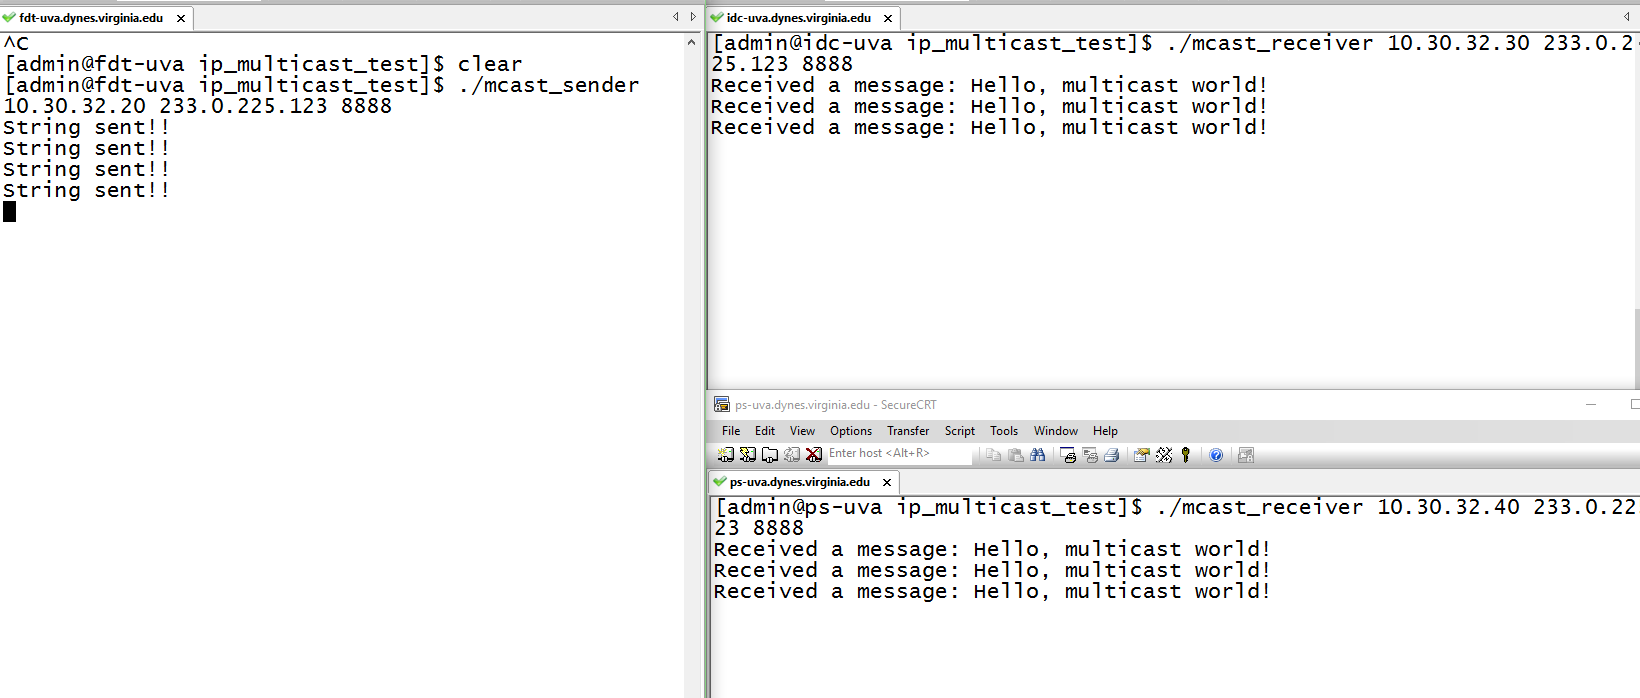
\includegraphics[width=0.8\textwidth]{figures/local-multicast.png}
\caption{UVA DYNES local multipoint experiment}
\label{fig:localmulticast}
\end{figure}

A GLOP multicast IP address is used for the multicast test. The 233.0.0.0/8 GLOP address IP range was assigned as experimental multicast address space for IP multicast service providers and network researchers. The middle two octets of this block are formed from assigned 16-bit autonomous system number (ASN). 233.0.225.123 is used since the ASN of UVA is 225.  When UVA FDT sent the multicast packets with message ``Hello, multicast world!'', IDC and pS hosts received the message at the same time. However, when we changed the VLAN tags of these 3 interfaces to different values in local OESS, the related flow entries were not set in the flow table of UVA DYNES switch since multipoint VLAN tag translation feature was not supported in Dell S4810 OpenFlow 1.0 switch.
\begin{figure}[htb!]
\centering
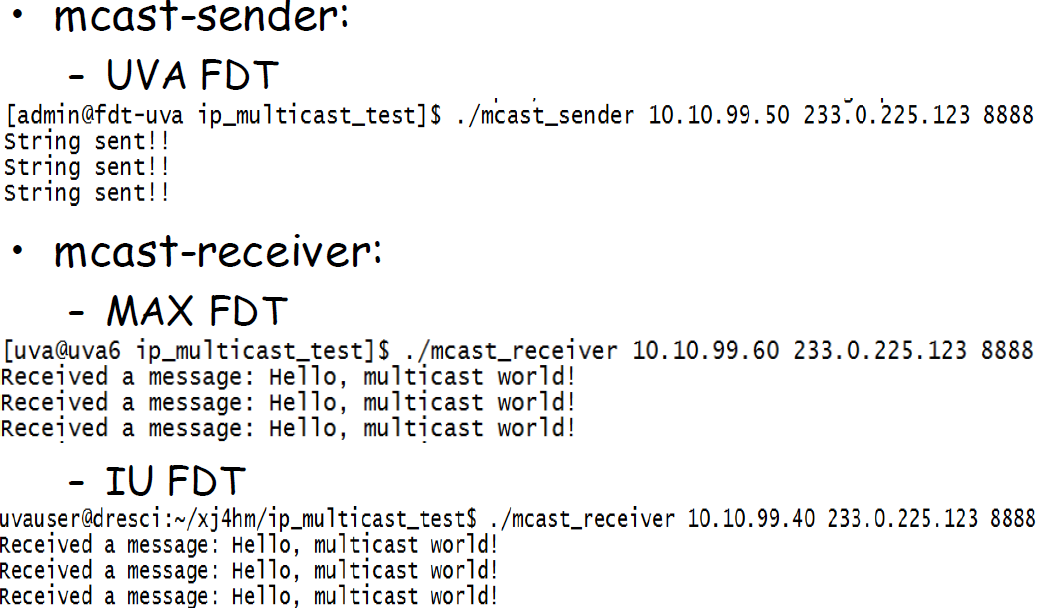
\includegraphics[width=0.8\textwidth]{figures/AL2Smulticast.png}
\caption{AL2S inter-domain multipoint experiment}
\label{fig:widemulticast}
\end{figure}


Finally, the inter-domain multi-point VLAN was tested by the IP multicast program. The control plane setup is described in Section~\ref{sec:controlplanefinal}. Fig.~\ref{fig:widemulticast} indicates the inter-domain multi-point VLAN is set up successfully. When UVA FDT was sending messages to the multicast group from the VLAN interface, both MAX FDT and IU FDT were receiving the ``Hello, multicast world!'' message at the same time.


\begin{figure}[htb!]
\centering
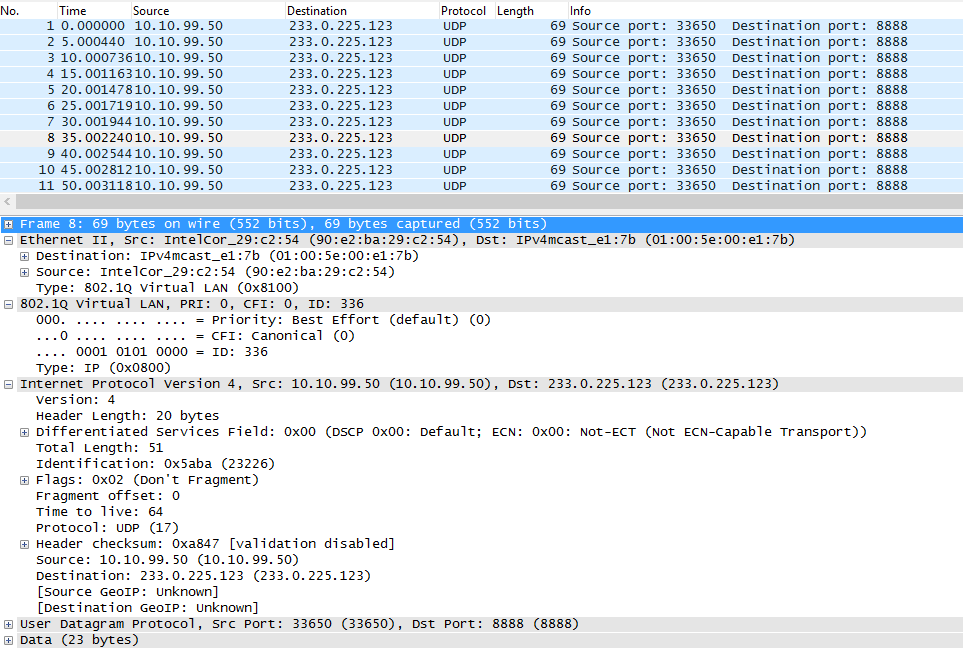
\includegraphics[width=0.8\textwidth]{figures/pcap.png}
\caption{Wireshark packets details of a pcap file}
\label{fig:pcap}
\end{figure}

For verifying the experiment was multicasting over the inter-domain multi-point VLAN, packets were captured by \texttt{tcpdump} utility for analyzing purpose. Fig.~\ref{fig:pcap} shows the detailed packets information of the inter-domain multicast experiment. The pcap file was captured in UVA FDT VLAN 336 interface whose 802.1q VLAN ID is 336. The destination IP address 233.0.225.123 is the GLOP multicast IP address we used for the test. The destination MAC address is 01:00:5e:00:e1:7b which is mapping with the GLOP IP address. As Fig.~\ref{fig:mapping} the hard-wired mapping solution for multicast IP address is used. For unicast IP addresses, ARP is used to find the corresponding MAC address, because an IP address corresponds to a host (also one MAC address for one host). However, for multicast IP address , one multicast IP address (Class-D) is for a group of hosts in the multicast group, this group shares one multicast MAC address. All multicast receivers need to “accept” Ethernet frames with a given destination MAC address. Without multicast, each Ethernet NIC will only accept Ethernet frames whose destination MAC address equals its own unicast MAC address and frames with destination MAC address equal to FF:FF:FF:FF:FF:FF (broadcast). So when mcast code issues the ipm socket system calls, the code calls the Ethernet driver to add another entry: 01:00:5e:00:00:F5 to accept frames with this destination MAC address. Since a multicast frame needs to be accepted by all receivers, we can have only one multicast MAC address corresponding to a group. The multicast address mapping verified the experiment was multicasting over the multi-point VLAN.


\begin{figure}[htb!]
\centering
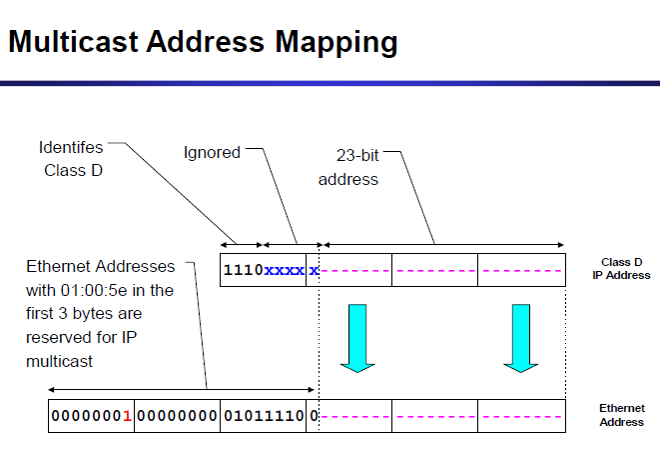
\includegraphics[width=0.8\textwidth]{figures/mapping.png}
\caption{Multicast address mapping}
\label{fig:mapping}
\end{figure}


\paragraph{Key Findings}
The key finding of the experiments are (i) Multipoint VLAN with different VLAN tags cannot be provisioned by OpenFlow 1.0 supported switches, but AL2S switches support this feature. Thus, inter-domain multi-point VLAN service from AL2S can be used for wide-area multicast applications. (ii) Packets with the multicast destination IP address might be dropped by firewall in some regional networks.


\section{Conclusions}
This chapter described our experience in deploying a multi-domain SDN and testing
a dynamic Layer-2 (L2) path service across this SDN. Our work demonstrated that inter-domain L2 paths can be created and released automatically, i.e., without administrator involvement, by using distributed per-domain SDN controllers.
We offered insights into this complex deployment process
and identified modifications required to the protocols and controllers
for improved user experience and scalability of this dynamic L2 path service.

%%%Talk about the multipoint VLAN 